\documentclass[11pt, a4paper]{article}
\usepackage[utf8]{inputenc}
\usepackage{fullpage}                                       %Changes the margin
\usepackage{fancyhdr}
\usepackage{graphicx}
\usepackage{fontspec}
\usepackage{setspace}
\usepackage{hyperref}

% \usepackage[margin=1in,headheight=100pt,headsep=0.3in,includehead]{geometry}

% \usepackage{geometry} 
% \geometry{a4paper, 
%             textwidth = 5.5in, 
%             textheight = 8.5in,
%             marginparsep = 7pt,
%             marginparwidth = .6in}

% \usepackage[usenames,dvipsnames]{color}
% \usepackage{xunicode}
% \usepackage{xltxtra}

% \setstretch{1.25}
\defaultfontfeatures{Mapping=tex-text}
\setmainfont[
        BoldFont = {Libertine_bold.ttf},
        ItalicFont = {Libertine_italic.ttf},
    ]{Libertine.ttf}
\hypersetup{
    colorlinks = true,
}
% \pagestyle{fancy}

% Headers - all currently empty
% \lhead{}
% \chead{}
% \rhead{}

% \renewcommand{\headrulewidth}{0.0pt}                        %No header rule
% \renewcommand{\footrulewidth}{0.4pt}                        %Thin footer rule

\begin{document}
\onehalfspacing
% \noindent\raisebox{0mm}[0pt][0pt]{\rlap{\makebox[\textwidth][r]{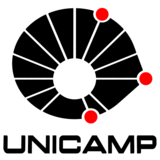
\includegraphics[height=15mm]{logo-unicamp-name.png}}}}
% \vspace{5mm}
% \noindent\raisebox{0mm}[0pt][0pt]{\rlap{\makebox[\textwidth][l]{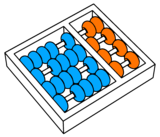
\includegraphics[height=15mm]{logo-ic-unicamp.png}}}}
% \vspace{5mm}

\hfill \textbf{\Large{Carta de apresentação}} \hfill \today
\newline
\newline
Meu nome é Luciana de Aguiar Sena e sou formada em Engenharia da Computação pela Universidade Federal do Amazonas. Eu participei do treinamento de circuitos integrados \href{http://www.ci-brasil.gov.br/index.php/pt/}{CI Brasil} e atualmente estou trabalhando no \href{https://www.eldorado.org.br}{Instituto Eldorado} em Campinas no Departamento de \textit{Hardware Design} na área de Verificação de Circuitos Integrados.

Durante a faculdade desenvolvi um grande interesse pela área de Aprendizagem de Máquina, especialmente em Reconhecimento de Padrões. Fiz Iniciação Científica (PIBIC) por 2 anos no tema de Reconhecimento de Padrões em Sinais de Vídeos Utilizando Detectores por Produto Interno, onde a proposta era o desenvolvimento de um detector que utilizava técnicas de filtragem por correlação e avaliar seu desempenho utilizando uma plataforma de hardware (Raspberry Pi).

Esse interesse e projeto acabou me levando ao mesmo tema no trabalho de conclusão de curso, onde continuei a trabalhar na pesquisa sobre detectores por produto interno no cenário de detecção de pontos fiduciais. Este trabalho me permitiu estudar mais a fundo sobre filtragem por correlação e ter um contato inicial com a biblioteca OpenCV e C++.

Além de todos os projetos, vida acadêmica, aprendizado de linguagens, o inglês também foi e tem sido um fator importante nos estudos, uma vez que muitos artigos, muitos livros e muitos guias utilizam da linguagem mundial para transmitir conhecimento. Eu estudei e conclui o curso de inglês na escola Cultura Inglesa, além de ter realizado um exame de Cambridge (\href{https://www.cambridgeenglish.org/exams-and-tests/key/}{KET}) antes de ter começado a graduação.

Também participei de alguns treinamentos durante a graduação como, por exemplo, o de Desenvolvimento de Sistemas de Processamento Digital de Imagens, onde tive contato com visão computacional, processos estocásticos, reconhecimento de padrões, processamento digital de imagens, classificação, aprendizado supervisionado etc. O projeto desenvolvido foi no tema de detecção de objetos abandonados, onde utilizamos um pouco de OpenCV e Python.

Outro foi na área de TV Digital interativa patrocinada pela Samsung, onde foi visto módulos como Java, C++, introdução a TV Digital, NCL, Lua, UML, transmissão digital, sistemas embarcados, \textit{device drivers} etc. O projeto desenvolvido para esse treinamento foi um aplicativo interativo sobre pontos turísticos do Brasil para TV Digital utilizando NCL.

Durante a graduação também tive a oportunidade de cursar Redes Neurais e Processamento Digital de Imagens (matérias da pós-graduação) como optativas e isso me deu uma base boa quando comecei a estudar sobre Deep Learning. 

Até o presente momento, já trabalhei com algumas linguagens (especialmente durante a faculdade), como C e Java primariamente. Um exemplo de projeto foi o desenvolvimento de um sistema de biblioteca em Java com uma versão Web feita em JavaScript. Entretanto, como atualmente estou cursando o \href{https://br.udacity.com/course/deep-learning-nanodegree-foundation--nd101}{Nanodegree de Deep Learning} da Udacity e alguns cursos relacionados a Machine Learning, comecei a trabalhar mais com Python, especialmente com as bibliotecas NumPy e Pandas. 

\begin{center}
\textbf{\small{Luciana Sena}}

\href{mailto:luciana.aguiar.sena@gmail.com}{\footnotesize luciana.aguiar.sena@gmail.com}

\footnotesize{(19) 98164-7268}
\end{center}
\end{document}
